%=== CHAPTER THREE (3) ===
%=== (Actual work done and contribution, including literature survey) ===


\begin{spacing}{2.0}
%\setlength{\parskip}{0.2in}
%  (Actual work done and contribution, including literature survey)


\section{Research Methodology}

Reid Mcllroy-young et al adopt a multi-step approach that involves feature extraction, aggregation at move and game levels, and player-level aggregation. The specific methodologies employed include the use of residual blocks for feature extraction, transformer-based methods for move-level to game-level aggregation, and centroid calculation for player-level aggregation \cite{stylometryChess}. 

Krizhevsk et al undertook an experimental approach toward image classification utilizing convolutional neural networks \cite{ImageClass}. In another study, the grounded theory approach was used to present its usefulness in agile development when it comes to the human and social elements of software development \cite{agileGrounded}.

\subsection{Academic Material and Non-Academic Material}

Although the distinction between academic and non-academic material is not always absolute, and there can be variations and overlap between the two categories, the below list offers my subjective view between the two definitions. 

\subsection{Academic Material}

Peer-Reviewed Journals: Academic material is often published in peer-reviewed journals. These journals follow a rigorous review process where experts in the field evaluate the quality and validity of the research before publication. Articles in peer-reviewed journals typically include original research, methodology, results, and discussion sections.

Scholarly Books: Academic material can be found in scholarly books published by reputable academic publishers. These books often present in-depth research, theoretical frameworks, and scholarly analysis of a specific topic.

Conference Proceedings: Research presented at academic conferences is often compiled in conference proceedings. These proceedings contain scholarly papers and presentations that undergo a review process before acceptance.

Theses and Dissertations: Academic material includes research conducted by graduate students in the form of theses and dissertations. These documents provide detailed studies on specific research topics and are often available through university repositories or libraries.

Academic Websites and Databases: Universities and research institutions often provide access to online databases, libraries, and repositories that host academic material. These platforms may include scholarly articles, conference papers, theses, and other research outputs.

\subsection{Non-Academic Material}

Popular Magazines and Newspapers: Non-academic material can be found in popular magazines, newspapers, and news websites. These sources typically provide general information, news, and feature articles targeting a broad audience.

Trade Publications: Industry-specific trade publications cater to professionals in specific fields or industries. They often cover industry trends, practical advice, and case studies relevant to professionals working in a specific domain.

Blogs and Online Forums: Non-academic material includes blogs and online forums where individuals share personal opinions, experiences, and insights. While they can offer valuable perspectives, they may lack the rigorous research and peer review found in academic material.

Websites and Social Media: Websites and social media platforms host a wide range of non-academic content. While they can provide information, news, and opinions, it is essential to critically evaluate the credibility and reliability of the sources and content shared.

Books and Publications for the General Public: Non-academic material includes books and publications intended for the general public. These books may offer popular science explanations, self-help advice, biographies, memoirs, and other forms of entertainment or information.

\subsection{Article Recommendations}

The most important articles in relation to this research area were undertaken by Mcllroy-young et al\cite{stylometryChess} which dramatically improved upon previous work in the field. The researchers work has been invaluable to my area of study, also publishing articles attempting to capture the human element in chess \cite{SuperAI}\cite{McIlroyYoung_Learning_Models_Chess_2022}. The aforementioned articles surprisingly managed to extract the human element from chess games and created a new human like model. Although niche, it has been a growing concern with the evolution of chess engines that they feel too robotic and inhuman when played against,
which in turn creates a feeling of frustration in the player.

They also explored ethical concerns regarding AI that mimic human behaviour \cite{mimicAI}. In another paper, researchers evaluate the capabilities of AlphaGo, AlphaGo Zero, and AlphaZero algorithms, showcasing the promising capabilities of self-learning algorithms \cite{alphazero}.

\begin{figure}[ht]
\centering
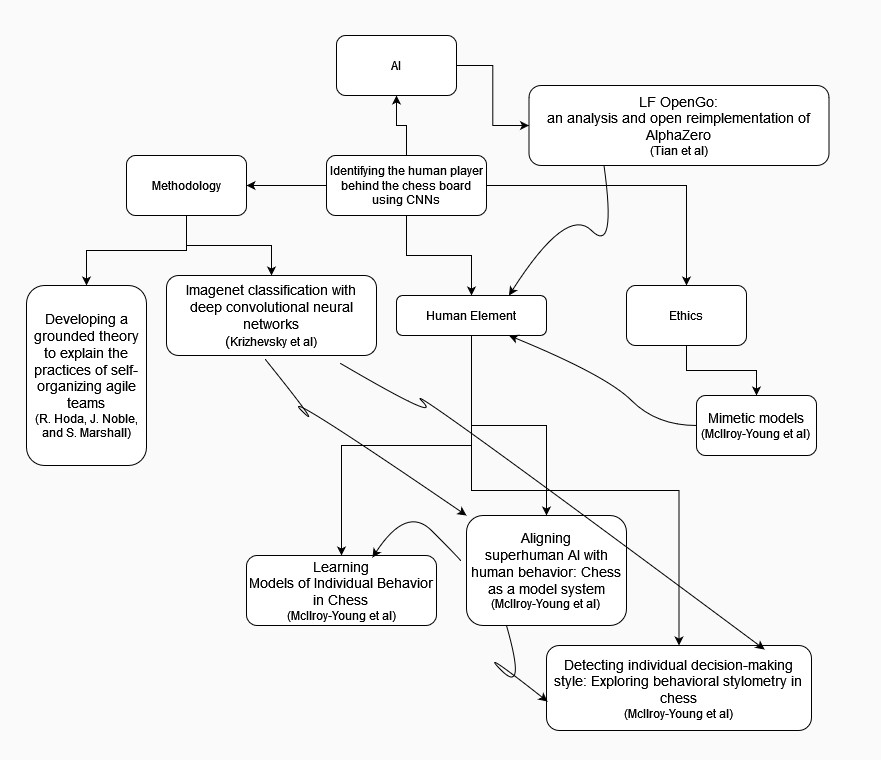
\includegraphics[scale=0.3]{Figures/LiteratureMap.jpg}
\caption{Literature Map}
\label{fig:LitMap} 
\end{figure}

\subsection{Contextualized literature and research material}

Contextualized literature and research material refers to scholarly works that are specifically situated within a particular context or setting, taking into account the specific variables, conditions, and factors that influence the subject of study. It goes beyond general academic sources and encompasses literature and research that is directly relevant, applicable, and specific to a particular context or field of study.

This type of material offers a deeper understanding of the subject matter by considering the unique circumstances, dynamics, and complexities within a given context. It acknowledges that different contexts can have distinct characteristics, influencing the way phenomena are understood, interpreted, and addressed. By examining literature and research that is contextualized, researchers can gain insights that are more meaningful, applicable, and tailored to their specific research questions or practical needs.

Contextualized literature and research material can include a variety of sources, such as specialized journals, case studies, field-specific books, government or institutional reports, and industry-specific research. These sources provide detailed analysis, empirical evidence, and theoretical frameworks that are directly relevant to the context under investigation. They often explore the interplay between various factors and variables specific to the context, shedding light on the unique challenges, opportunities, and dynamics that shape the subject of study.

By utilizing contextualized material, researchers can develop a nuanced understanding of the complexities within a particular context, enabling them to make informed decisions, propose targeted interventions, or generate knowledge that is applicable and relevant to the specific circumstances at hand. This type of literature and research material helps to bridge the gap between theory and practice by providing insights that are tailored to the specific context, leading to more effective and meaningful outcomes.


%=== END OF CHAPTER THREE ===
\end{spacing}
\newpage
